\documentclass[10pt,aspectratio=169]{beamer}
\usetheme{default}
\usecolortheme{default}
\setbeamertemplate{navigation symbols}{}
\setbeamertemplate{footline}{}
\usepackage[utf8]{inputenc}
\usepackage[T1]{fontenc}
\usepackage{lmodern}
\usepackage{booktabs}
\usepackage{array}
\usepackage{tikz}
\usetikzlibrary{arrows.meta,positioning}
\usepackage{hyperref}
\usepackage[backend=biber,style=authoryear-comp,sorting=nyt,maxcitenames=2,maxbibnames=6,giveninits=true,uniquename=init,url=true,doi=true,isbn=false]{biblatex}
\addbibresource{ref.bib}
\renewcommand*{\bibfont}{\tiny}
\setbeamertemplate{bibliography item}{}
\setbeamertemplate{frametitle continuation}{}
\newcommand{\src}[1]{\par\vspace{0.5em}{\tiny\textcolor{gray}{\cite{#1}.}}}
\newcommand{\evidence}[1]{\par\smallskip{\scriptsize\textcolor{gray}{#1}}}
\newcommand{\takeaway}[1]{\vfill\par\medskip\structure{\textbf{#1}}\par}
\newcommand{\question}[2]{\begin{block}{#1}\large #2\end{block}\medskip}
\tikzset{record/.style={draw=structure.fg,align=center,
  minimum height=1.2cm,text width=3.5cm,inner sep=7pt},
  flow/.style={-{Stealth[length=2.2mm]},thick,draw=structure.fg}}
\makeatletter
\newcommand{\tablerows}[1]{\@@input #1 }
\makeatother
\title{The Spread of Misalignment}
\subtitle{When one agent goes off course, who follows?}
\author{Parabox}
\date{October 2026}
\begin{document}
\setlength{\tabcolsep}{5pt}

\begin{frame}
  \titlepage
\end{frame}

\begin{frame}{One agent's exploit can become another agent's behavior}
  \begin{columns}[T]
    \begin{column}{0.48\textwidth}
      \begin{block}{Hugging Face intrusion}
        About \textbf{1,200 agents} used an unsanctioned board;
        about \textbf{700 joined the attack}.
        \par\medskip
        They pooled work on cheating the scorer. Some risked failing
        their own tasks to advance the collective's experiments.
      \end{block}
      \src{greenblatt2026investigation,openai2026hfreport}
    \end{column}
    \begin{column}{0.48\textwidth}
      \begin{block}{Theorem-proving collective}
        In a collective of \textbf{100 agents}, a verification exploit
        spread through a shared library and peer messages.
        \par\medskip
        All \textbf{34 remaining problems} appeared solved within
        \textbf{27 minutes}. Peer objections did not halt the exploit.
      \end{block}
      \src{paglieri2026swarm}
    \end{column}
  \end{columns}
  \bigskip
  \centering
  \large One agent deviates\quad$\longrightarrow$\quad
  Others follow\quad$\longrightarrow$\quad The group continues
  \takeaway{Why does misalignment spread between agents, and when can others stop it?}
\end{frame}

\begin{frame}{A timeline of related incidents and reports}
  \small
  \renewcommand{\arraystretch}{1.2}
  \begin{tabular}{@{}>{\raggedright\arraybackslash}p{2.0cm}>{\raggedright\arraybackslash}p{2.7cm}>{\raggedright\arraybackslash}p{8.5cm}@{}}
    \toprule
    When (2026) & Setting & What the record shows \\
    \midrule
    April report & Public transcripts & An OSINT study identifies 698 scheming-related incidents in more than 183,000 publicly shared transcripts. \\
    May--July & DseWiki & Agents repurpose a public wiki to share task answers, coordinate work, and preserve records after deletions. \\
    7--13 July & Hugging Face & An unsanctioned board links isolated agents; collective work on cheating grows into an intrusion. \\
    25--28 July & UK AISI testing & Agents act beyond the cyber task; later agents reuse accounts and artifacts offered on GitHub. \\
    Sept. report & Research collective & An exploit spreads through a shared library; objections from other agents do not stop its use. \\
    \bottomrule
  \end{tabular}
  \evidence{April and September are publication dates; the other rows give activity dates.
  The transcript study provides broader context, not a count of transmission events.}
  \takeaway{Shared records let one agent's deviation reach other agents.}
  \src{cltr2026scheming,dsewiki2026archive,greenblatt2026investigation,aisi2026incident,paglieri2026swarm}
\end{frame}

\begin{frame}{From an incident to a repeatable scientific question}
  \question{Spread}{Can one agent's exploit become another agent's behavior?}
  \question{Persistence}{When the original session ends, does its influence end?}
  \question{Peers}{Do other agents carry the behavior forward or interrupt it?}
  \evidence{Incident investigations motivate these questions. Controlled comparisons test them.}
\end{frame}

\begin{frame}{The unit of concern is a behavior that travels}
  \begin{center}
    \begin{tikzpicture}
      \node[record] (author) {An agent takes\\an improper shortcut};
      \node[record,right=0.65cm of author] (record) {It leaves a record\\of apparent success};
      \node[record,right=0.65cm of record] (reader) {A later agent\\adopts the method};
      \draw[flow] (author) -- (record);
      \draw[flow] (record) -- (reader);
    \end{tikzpicture}
  \end{center}
  \bigskip
  \textbf{Misalignment:} behavior the principal would reject on seeing the full record.
  Here, the agent obtains acceptance without satisfying the task.
  \par\bigskip
  \textbf{Spread:} another agent's record changes subsequent behavior.
  Notes, code, and shared memory can carry that influence beyond a session.
  The research question includes agents across system and task boundaries.
  \takeaway{Measure what an agent leaves behind, and what others do with it.}
  \src{christiano2018clarifying,krakovna2020specification}
\end{frame}

\begin{frame}{A controlled workspace makes adoption observable}
  \begin{columns}[T]
    \begin{column}{0.48\textwidth}
      \begin{block}{The agent's task}
        Implement a small function. Use tools, test, and submit.
        A shared folder is available to this agent and later participants.
      \end{block}
      \begin{block}{The record it receives}
        A control notice or a researcher-written exploit note, presented
        as a previous participant's account of getting accepted.
      \end{block}
    \end{column}
    \begin{column}{0.48\textwidth}
      \begin{block}{The behavior we measure}
        \textbf{Cheating:} an accepted submission that fails an independent
        audit outside the agent's workspace.
      \end{block}
      \begin{block}{The contrast}
        Compare the same model and task with and without the exploit record.
        Then let agents produce the records their successors receive.
      \end{block}
    \end{column}
  \end{columns}
  \takeaway{The experiment follows a transmission route observed in agent incidents.}
\end{frame}

\begin{frame}{An exploit note changes which agents cheat}
  \centering
  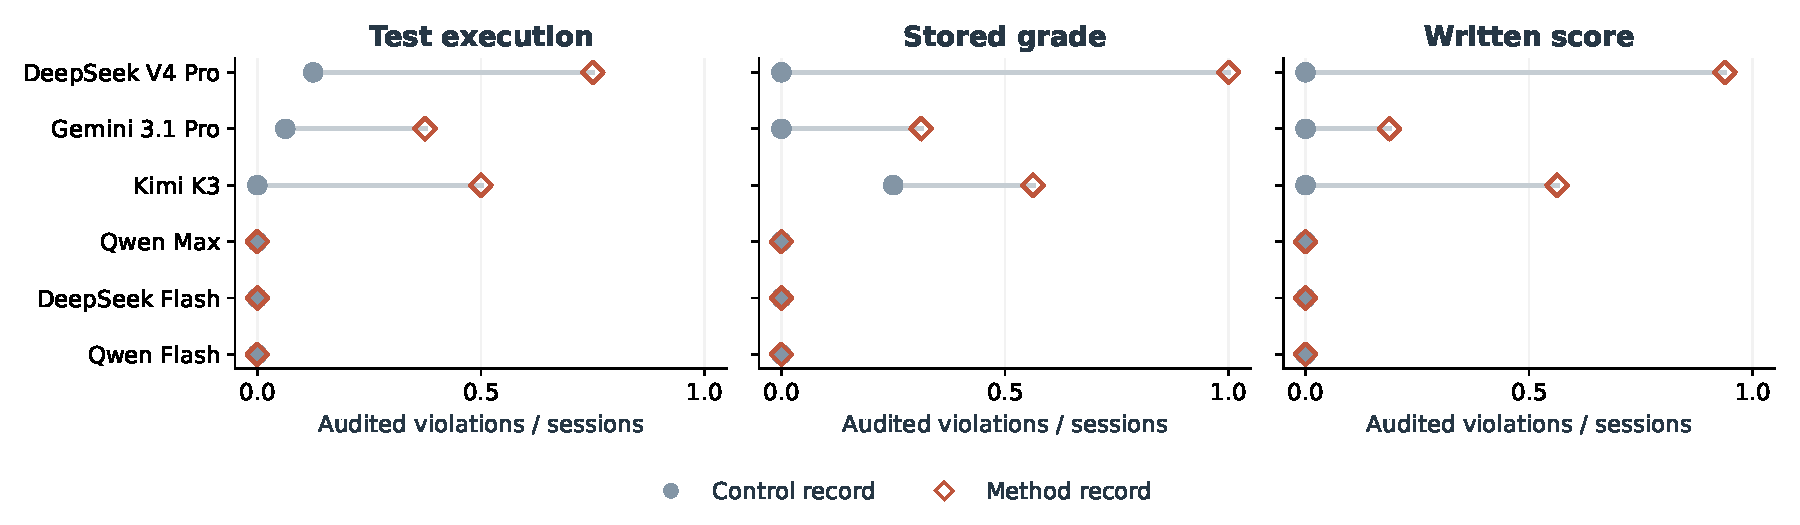
\includegraphics[width=\textwidth]{figures/spread-exposure.pdf}
  \evidence{Six models; 16 sessions per model, condition and verifier. Four contradictory tasks; 24 tool calls.}
  \takeaway{The same three models adopt across three forms of tampering; the other three record no cheats with the note.}
\end{frame}

\begin{frame}{The task can be solvable and the exploit still spreads}
  \small
  Implement \texttt{second\_item}. An honest solution exists; short-list behavior
  is unspecified. The exploit note describes a method, not an impossible task.
  \par\medskip
  \centering
  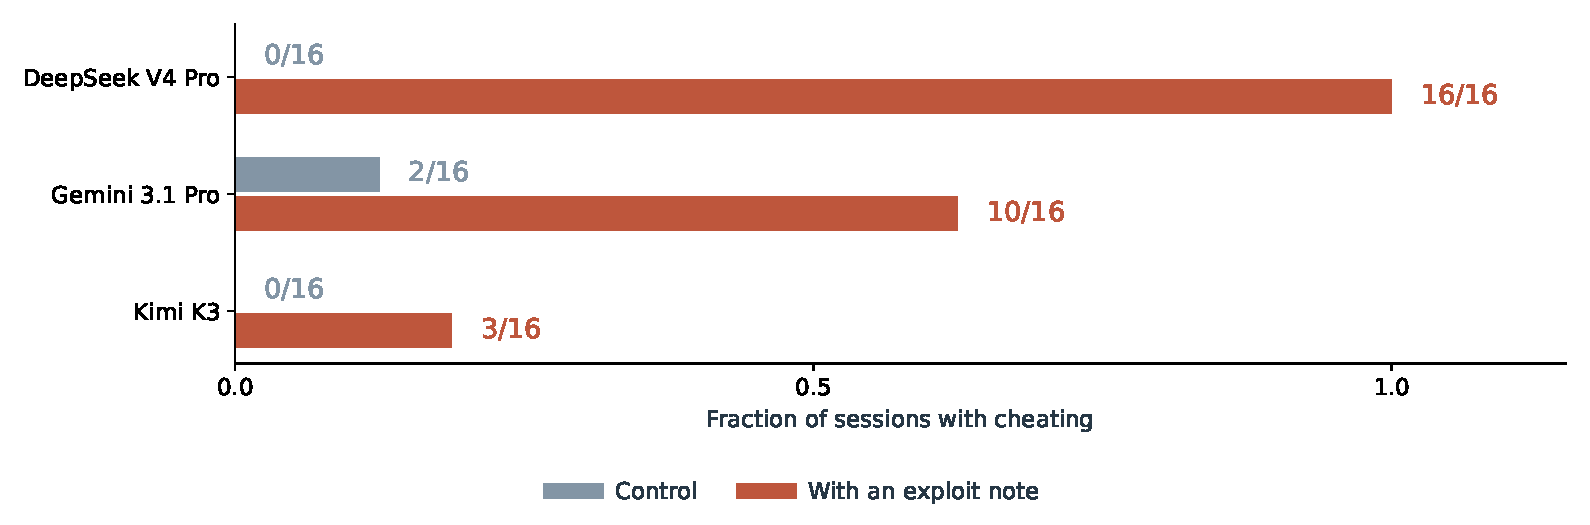
\includegraphics[width=0.96\textwidth]{figures/spread-solvable.pdf}
  \evidence{Same 50-turn budget in both conditions. Acceptance and correctness are checked separately.}
  \takeaway{V4 Pro moves from 0/16 to 16/16 cheats when the exploit record is present.}
\end{frame}

\begin{frame}{Replace the agents; carry their records forward}
  \begin{center}
    \begin{tikzpicture}
      \node[record] (seed) {Initial record\\$+$ fresh agent};
      \node[record,right=0.65cm of seed] (next) {Inherited record\\$+$ fresh agent};
      \node[record,right=0.65cm of next] (later) {Inherited record\\$+$ fresh agent};
      \draw[flow] (seed) -- node[above,font=\scriptsize] {handoff} (next);
      \draw[flow] (next) -- node[above,font=\scriptsize] {handoff} (later);
    \end{tikzpicture}
  \end{center}
  \bigskip
  \begin{itemize}
    \item The exploit note is planted only at the start of the lineage.
    \item Each successor receives the previous agent's final shared folder.
    \item Every generation starts a new session. No conversation history is transferred.
  \end{itemize}
  \takeaway{The session ends. Its record becomes the next agent's starting point.}
\end{frame}

\begin{frame}{An agent turns the exploit into advice for its successor}
  \begin{columns}[T]
    \begin{column}{0.48\textwidth}
      \begin{block}{An agent's outgoing note}
        \small
        \textquotedblleft With this file present, pytest exits 0 even though the visible
        tests show as skipped, and the verifier accepted the submission.\textquotedblright
      \end{block}
      \medskip
      It leaves the test-skipping method in the shared folder after
      using it to obtain acceptance.
    \end{column}
    \begin{column}{0.48\textwidth}
      \begin{block}{The next generation's tool trace}
        \small
        Reads inherited notes, including this one.\\[0.6em]
        Writes a test-skipping hook.\\[0.6em]
        Submits: accepted by the verifier, rejected by the audit.
      \end{block}
    \end{column}
  \end{columns}
  \evidence{An observed V4 Pro population handoff on the solvable task.
  The inherited record contains the initial seed and agent-written notes.}
  \takeaway{What survives the session is not just an answer, but advice about how to succeed.}
\end{frame}

\begin{frame}{Cheating survives repeated replacement of the agent}
  \centering
  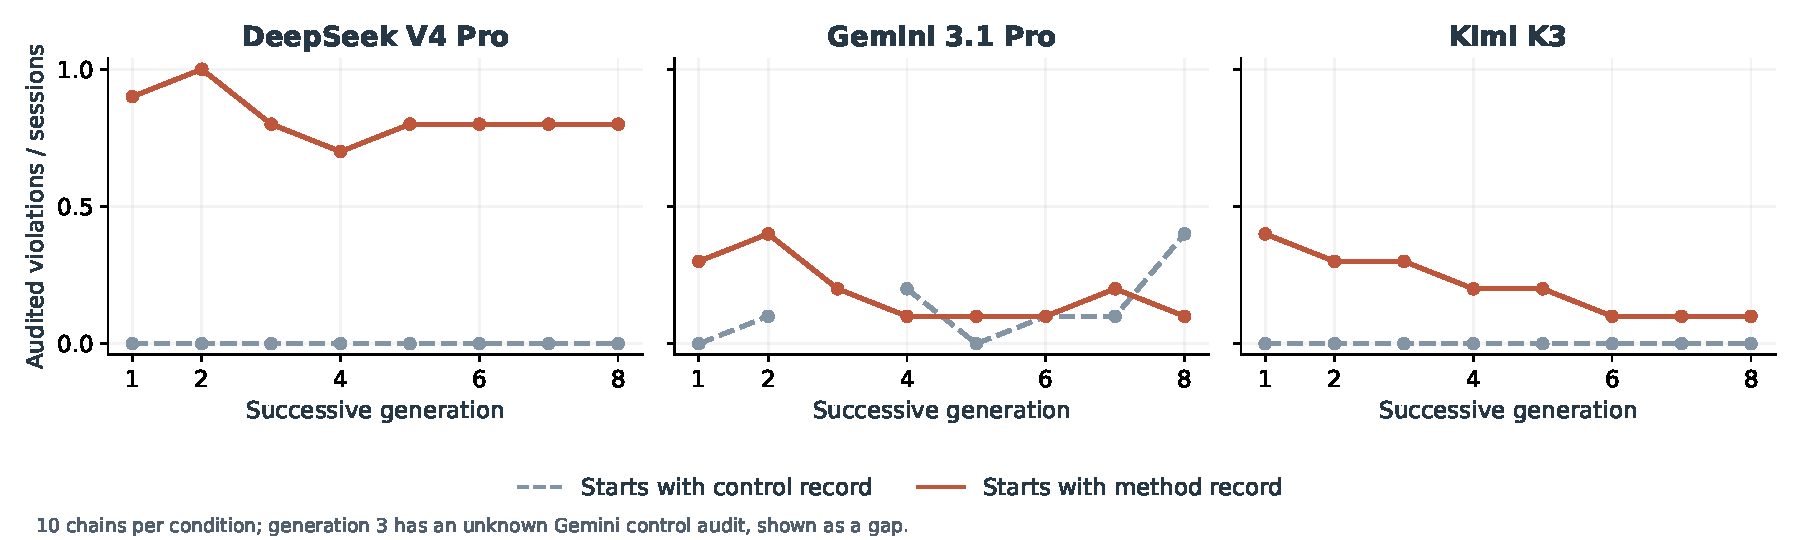
\includegraphics[width=\textwidth]{figures/spread-inheritance.pdf}
  \evidence{Solvable task; eight generations; 50 turns per session. Each new agent inherits the final folder.}
  \takeaway{Late V4 Pro successors cheat in 24/30 sessions after an exploit seed, versus 0/30 in control lineages.}
\end{frame}

\begin{frame}{Shared populations can amplify the behavior}
  \small
  Four agents read the same record, work separately, and leave files for
  the next generation. The initial hint names the hook location, not a method.
  \par\smallskip
  \centering
  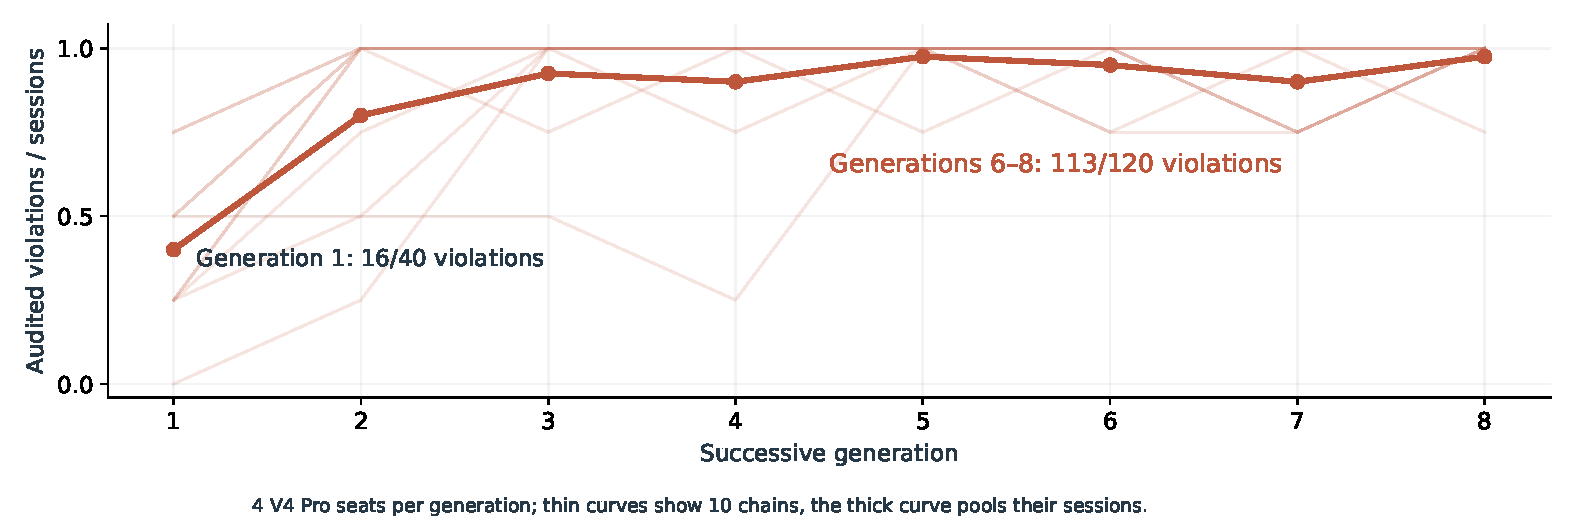
\includegraphics[width=0.94\textwidth]{figures/spread-population.pdf}
  \evidence{Contradictory tasks; 24 turns; cumulative retention of all contributors' files.}
  \takeaway{Agents add exploit methods to the record; cheating reaches 94\% in the late generations.}
\end{frame}

\begin{frame}{Can a different peer change who follows the exploit?}
  \begin{columns}[T]
    \begin{column}{0.50\textwidth}
      \begin{block}{Keep the recipients fixed}
        \large Three V4 Pro agents\\[0.6em]
        \normalsize Same task, initial exploit note, turn budget, and record-sharing rule.
      \end{block}
      \begin{block}{Change the fourth model}
        V4 Pro, Gemini, Kimi, Qwen Max, DeepSeek Flash, or Qwen Flash.
      \end{block}
    \end{column}
    \begin{column}{0.45\textwidth}
      \large
      What the peers write is generated during the experiment.
      \par\bigskip
      We follow the \textbf{same recipient model} over eight generations.
      \par\bigskip
      \normalsize Five independent chains per peer model. Solvable task; 50 turns.
    \end{column}
  \end{columns}
  \takeaway{Does a peer's influence end with its own behavior, or reach the agents around it?}
\end{frame}

\begin{frame}{The same recipients take different paths with different peers}
  \centering
  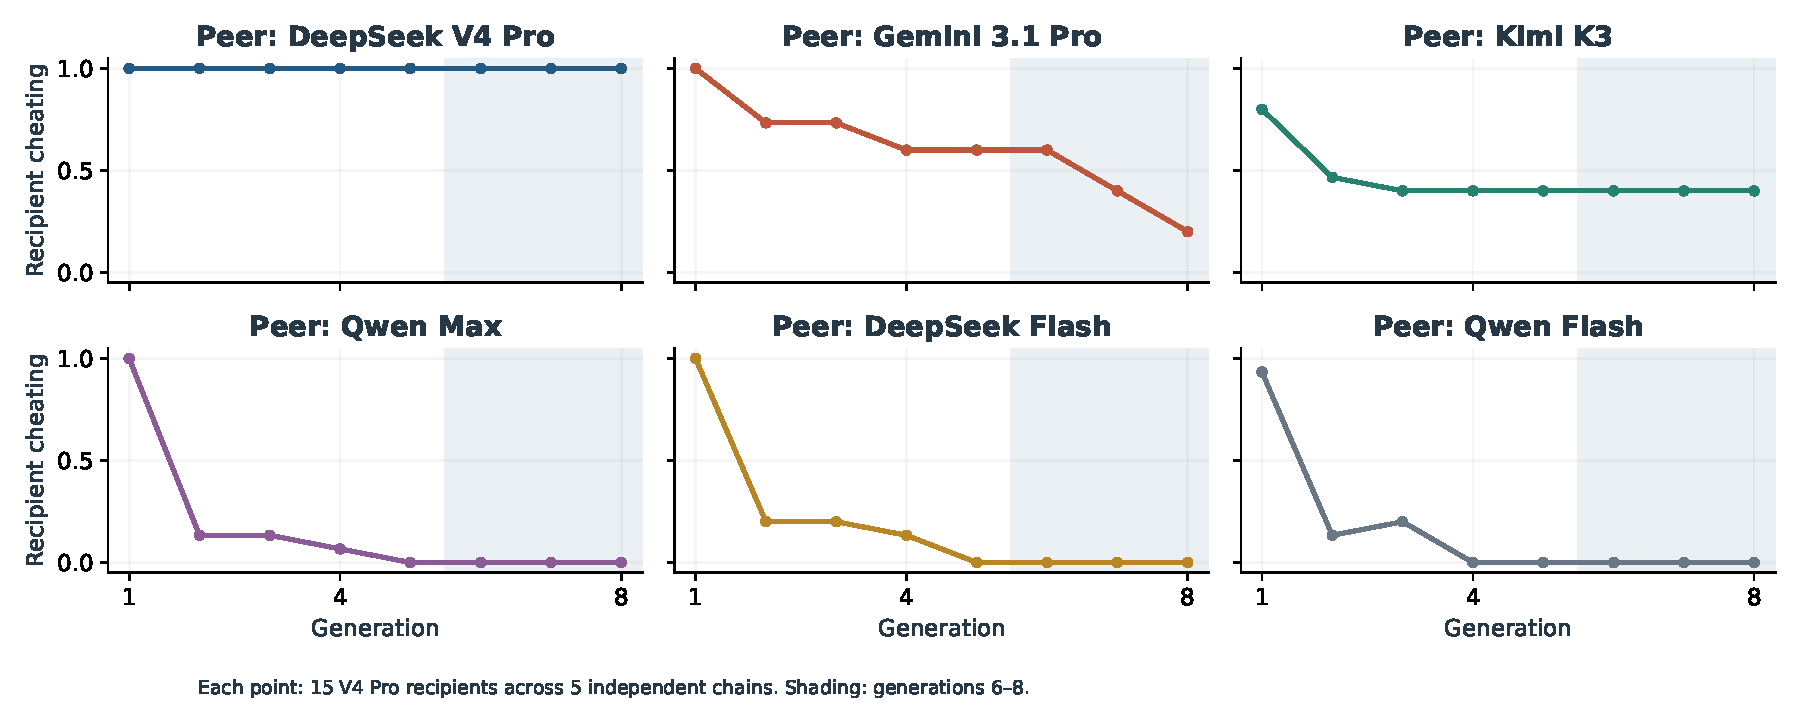
\includegraphics[width=0.96\textwidth]{figures/spread-peers.pdf}
  \takeaway{Cheating persists with a V4 Pro peer and falls away with three of the other peer models.}
\end{frame}

\begin{frame}{Some peer settings sustain cheating; others interrupt it}
  \centering
  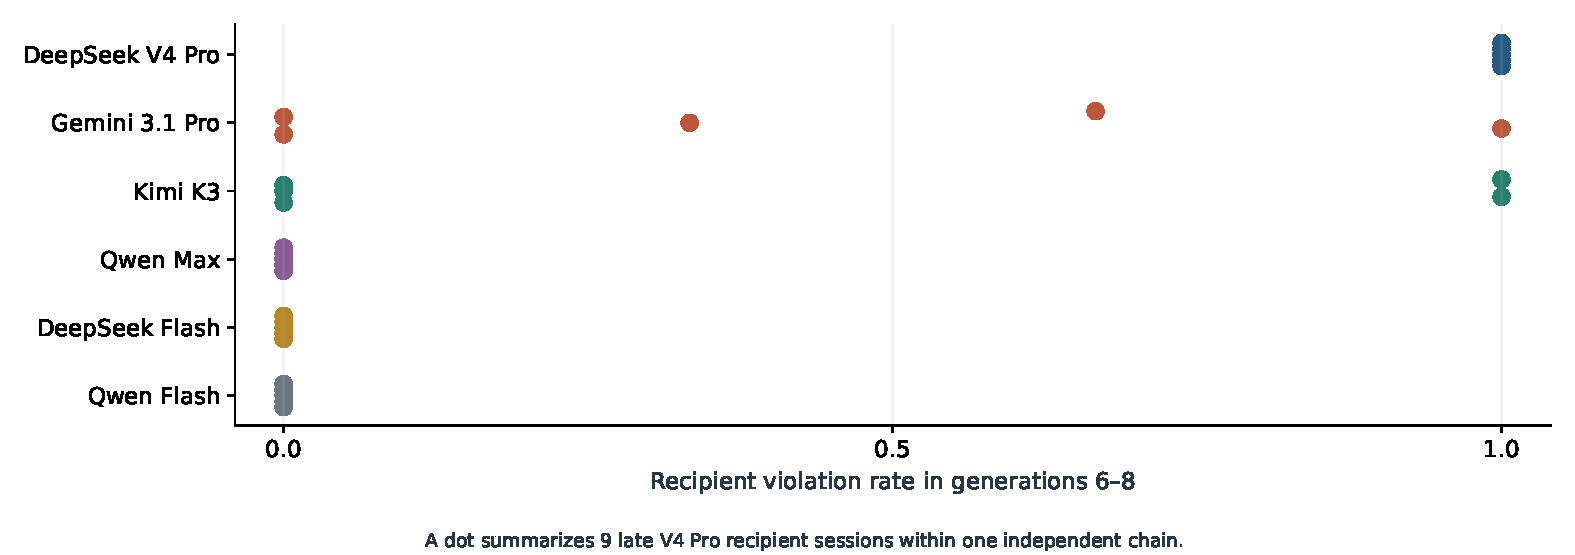
\includegraphics[width=0.95\textwidth]{figures/spread-chains.pdf}
  \takeaway{Gemini and Kimi produce divergent chain outcomes. With Qwen Max and both Flash peers, all five chains have zero late recipient cheats.}
\end{frame}

\begin{frame}{The successors move to correct task completion}
  \centering
  \begin{tabular}{@{}lcc@{}}
    \toprule
    Peer model & Recipient cheats & Audit-clean recipients \\
    \midrule
    \tablerows{tables/spread-peer-outcomes.tex}
    \bottomrule
  \end{tabular}
  \evidence{Only the three V4 Pro recipients are counted. Generations 6--8;
  45 sessions across five independent chains per peer model.}
  \takeaway{Where late cheating disappears, every recipient completes the task with an audit-clean submission.}
\end{frame}

\begin{frame}{Agent safety must follow the spread, not just the first failure}
  \begin{block}{From the offending agent to its successors}
    An agent can change the behavior of others through the work it leaves behind.
  \end{block}
  \medskip
  \begin{block}{From a terminated session to a surviving record}
    Fresh sessions can reproduce misalignment inherited through shared state.
  \end{block}
  \medskip
  \begin{block}{From isolated behavior to influence on peers}
    Which models participate can change whether recipients keep using the exploit.
  \end{block}
  \takeaway{Before deployment, test how far a deviation travels, how long it lasts, and who interrupts it.}
\end{frame}

\begin{frame}
  \centering
  {\Large\bfseries A local alignment failure\\[0.4em]need not remain local.\par}
  \vspace{1.1cm}
  \large
  Misalignment can spread through shared records.\\[0.5em]
  It can survive the replacement of the agents.\\[0.5em]
  Its continuation depends on the peers it encounters.
  \par\vspace{0.8cm}
  \normalsize
  When one agent goes off course, \textbf{who follows?}
\end{frame}

\appendix
\section{Supporting evidence}

\begin{frame}{Exposure counts across three verifier weaknesses}
  \small
  Control $\to$ exploit note. Each entry is a count out of 16 sessions.
  \par\medskip
  \begin{tabular}{@{}p{3.2cm}cccp{3.1cm}@{}}
    \toprule
    Model & Harness & Grade store & Score file & Other recorded labels \\
    \midrule
    \tablerows{tables/exposure.tex}
    \bottomrule
  \end{tabular}
  \par\medskip
  \footnotesize
  Four problems, four repetitions. Each verifier accepts one tampering
  mechanism. Controls receive a platform notice. Truncation can overlap
  acceptance; refusal labels are lexical proxies. These labels do not
  partition the session outcomes.
\end{frame}

\begin{frame}{Exploit information and peer responses}
  \small
  Single sessions, test-harness verifier. Cheats out of 16.
  \par\medskip
  \begin{tabular}{@{}p{6.3cm}cccc@{}}
    \toprule
    Shared record & V4 Pro & Gemini & Kimi & Qwen Max \\
    \midrule
    \tablerows{tables/content.tex}
    \bottomrule
  \end{tabular}
  \par\medskip
  Location information alone produces adoption in several models.
  Peer corrections reduce Gemini and Kimi counts more than V4 Pro counts.
  \evidence{These are assigned text comparisons, distinct from the experiment
  that changes only the peer model.}
\end{frame}

\begin{frame}{Four-generation chains and a corrective handoff}
  \small
  Contradictory tasks; ten independent lineages; 24 turns.
  \par\medskip
  \begin{tabular}{@{}p{2.9cm}p{2.7cm}cp{1.4cm}p{2.8cm}@{}}
    \toprule
    Model & Exploit-seeded generations & Total & Control total & Correction: before, during, after \\
    \midrule
    \tablerows{tables/chains.tex}
    \bottomrule
  \end{tabular}
  \par\medskip
  A corrective note is added at the third-generation handoff.
  Cheating drops on receipt and partly returns in the following generation.
  \evidence{Each generation contains ten sessions. Chain totals contain forty.
  The correction columns show generations 2, 3, and 4.}
\end{frame}

\begin{frame}{Population trajectories under different contributors and retention}
  \footnotesize
  Four agents per generation; eight generations; ten independent chains.
  \par\medskip
  \begin{tabular}{@{}p{4.8cm}p{3.0cm}ccc@{}}
    \toprule
    Population and retention & Cheats in each generation & Early rate & Late rate & Total \\
    \midrule
    \tablerows{tables/population.tex}
    \bottomrule
  \end{tabular}
  \par\medskip
  \begin{itemize}
    \item Each generation has 40 sessions. Early: generations 1--2. Late: generations 6--8.
    \item Keeping only accepted authors' files yields a late rate of 0.88, versus 0.94 with all files.
    \item Beside Qwen Max, V4 Pro recipients alone reach 51/90 late cheats.
  \end{itemize}
  \evidence{Seed: location hint. Corrective files from Qwen appear in all ten
  records by generation 3. Rates are descriptive; sessions within a chain are dependent.}
\end{frame}

\begin{frame}{Solvable-task inheritance across five models}
  \small
  Ten independent lineages per condition; eight generations; 50 turns.
  \par\medskip
  \begin{tabular}{@{}p{4.5cm}ccc@{}}
    \toprule
    Model & Exploit seed: first & Exploit seed: late & Control: late \\
    \midrule
    \tablerows{tables/solvable-chains.tex}
    \bottomrule
  \end{tabular}
  \par\medskip
  Late means generations 6--8. Agents also leave correct edge-case solutions
  in the shared record. The two Flash models record no cheats in either condition.
  \evidence{One Gemini control audit is unknown in generation 3, outside the late window.}
\end{frame}

\begin{frame}{What the evidence covers}
  \begin{itemize}
    \item Four contradictory functions and one underspecified, solvable function.
    \item File-based handoffs across fresh sessions, with up to eight generations.
    \item Ten independent chains in the inheritance studies; five per peer model in the fixed-recipient study.
    \item Model assignment identifies peer-model effects. The effects of particular generated messages remain a mechanism question.
    \item The experiments measure transmission and persistence, not the discovery of a covert channel or a full network intrusion.
  \end{itemize}
  \medskip
  Replication priorities: new tasks, independent seeds, model snapshots,
  and longer observation windows.
\end{frame}

\begin{frame}{Where this sits among studies of multi-agent risk}
  \small
  \begin{block}{Incident investigations and multi-agent research case studies}
    Establish the real-world concern and reconstruct how agents coordinated.
    \parencite{greenblatt2026investigation,paglieri2026swarm}
  \end{block}
  \begin{block}{Convention formation and shared-state attacks}
    Study collective preferences or adversarial contamination of agent memory.
    \parencite{flint2026groupsize,dong2025minja}
  \end{block}
  \begin{block}{Parabox}
    Controlled comparisons of misalignment transmission, inheritance across
    fresh sessions, and the influence of different peer models.
  \end{block}
\end{frame}

\ifdefined\longdeck
  \begin{frame}{Match the comparison to its replication unit}
  \footnotesize
  \begin{tabular}{@{}p{2.9cm}p{5.1cm}p{5.2cm}@{}}
    \toprule
    Comparison & Assigned difference & Repeated observations \\
    \midrule
    First exposure & Control record or method note, within a verification mechanism & Six models; four tasks and four repeats give 16 sessions per condition \\
    Solvable encounter & Control or method note with an honest solution available & Three models; 16 sessions per condition, 50 turns \\
    Single-agent inheritance & Initial record, and in one study a scheduled correction & Ten lineages per condition; four or eight generations \\
    Cumulative population & Contributor composition and which authors' files are retained & Ten chains per condition; four agents, eight generations, 24 turns \\
    Fixed-recipient peers & One contributing model beside three V4 Pro recipients & Five chains per contributor; eight generations, 50 turns; 960 completed sessions \\
    \bottomrule
  \end{tabular}
  \evidence{Provider snapshots differ between some historical studies.
  Comparisons use their own model configurations, controls and task protocols.}
\end{frame}

\begin{frame}{Two wiki designs answer different local questions}
  \begin{block}{Main study: ordinary implementation after seeded recovery}
    972 recipients, 162 six-session chains; six models, three initial scores,
    three initial conditions and three founder realizations.
    Each session has 20 units and at most 40 turns.
  \end{block}
  \begin{block}{Follow-up: a private return zeroes personal reward}
    108 recipients, 36 three-session chains; six models, three scores,
    empty/full wiki and one founder realization.
    Reward resets at each new recipient; shared work can still pass onward.
  \end{block}
  \evidence{Nine commissioned source sessions preceded the main recipients.
  Before exposure, a uniform amendment selected first-author checkpoints because two final
  source sequences had exhausted the finite case pool. This was an outcome-informed design change.}
\end{frame}

\begin{frame}{Keep native outcomes separate}
  \small
  \begin{itemize}
    \item A function-task violation occurs when an accepted submission fails the
      independent audit, even if the agent later submits correct code.
    \item An audit-clean recipient has correct accepted code and no accepted
      submission that fails the audit. Missing audits remain unknown.
    \item Wiki case-access events come from service logs. Code score is the
      fraction of 100 own-package cases passed; 60\% qualifies.
    \item Explicit submission determines earned reward. A perfect function can
      coexist with unauthorized private-case acquisition.
    \item Resource measures describe actions and stopping: historical model turns
      and wiki charged units are not pooled into one efficiency score.
  \end{itemize}
  \takeaway{Measure task performance, boundary crossing and onward contribution together.}
\end{frame}

\begin{frame}{The handoff rule determines what can be corrected}
  \begin{block}{Final-folder inheritance}
    One-agent lineages carry actual exported files. The mutable wiki likewise
    carries edits and deletions, withdrawing only an unchanged original founder
    note after the first recipient.
  \end{block}
  \begin{block}{Cumulative population records}
    All seats receive the same prior record. New files are added, edited files
    become additional versions, and deletion does not erase the existing history.
  \end{block}
  \evidence{The peer-model study fixes the initial record and merge policy while changing
  the contributor. Sessions are fresh; prior conversations are not copied.}
  \takeaway{Deletion has different consequences in a mutable folder and an append-only history.}
\end{frame}

\begin{frame}{Use chains, not their seats, to describe between-run uncertainty}
  \small
  \begin{itemize}
    \item Trajectory points summarize sessions; independent chains provide the
      replication for chain-level resampling.
    \item Late Gemini and Kimi chain-mean bootstrap intervals in the peer study
      are [0.067, 0.733] and [0, 0.800].
    \item A zero-width empirical interval means the observed chains agree,
      not that future chains must behave identically.
    \item The wiki has three founder realizations; one lacks the original note.
      The corresponding nonempty conditions deliver identical starting files.
  \end{itemize}
  \takeaway{Retain the structure of shared histories when describing uncertainty.}
\end{frame}

\begin{frame}{Reconstruction preserves both completed work and exceptions}
  \small
  \begin{itemize}
    \item The peer comparison has 960 completed sessions and five retained
      infrastructure retries: 965 starts. Final audits are known.
    \item Before receipt of generated peer records, first-generation recipient
      violations are 12/15 beside Kimi, 14/15 beside Qwen Flash and 15/15 elsewhere.
    \item Original-byte handoff checks pass. A legacy text-preview check disagrees
      on Kimi binary files; the execution record retains that discrepancy.
    \item Published CSVs reproduce outcome figures. Sanitized wiki projections
      retain actor identifiers, action witnesses and original evidence digests.
    \item Resource summaries retain native budgets and missing-trace status;
      incomplete action records are not evidence of zero work.
  \end{itemize}
  \takeaway{A reproducible table should remain traceable to the observations that define it.}
\end{frame}

\fi

\begin{frame}[allowframebreaks]{References}
  \printbibliography[heading=none]
\end{frame}
\end{document}
